\documentclass[draft,ras]{Template/AGUTeX}

\usepackage{graphicx}   % if you want to include graphics files
\usepackage{subfigure}
\usepackage{setspace}
\usepackage{amsxtra}
\usepackage{amsmath}
\usepackage{amssymb}
\usepackage{multirow}
\usepackage{bm}

% graphics path
\graphicspath{{Figs/}}

\authorrunninghead{SWOBODA ET AL.}
\titlerunninghead{3-D ISR}


\authoraddr{Corresponding author: J. P. Swoboda,
Department of Electrical \& Computer Engineering,
Boston University, 8 Saint Mary�s Street
Boston, MA 02215, USA.
(swoboj@bu.edu)}

\begin{document}

\title{Space-Time Ambiguity Function in 3-D ISR}
%%%%%%%%%%%%%% Author Info %%%%%%%%%%%%%%%%%%%%%%%%%%%%%%%%%%%%%
\authors{John Swoboda,\altaffilmark{1}
Joshual Semeter,\altaffilmark{1} Philip Erickson \altaffilmark{2}}

\altaffiltext{1}{Department of Electrical \& Computer Engineering,
Boston University, Boston, Massachusetts, USA.}
\altaffiltext{2}{Atmospheric Science Division,
MIT Haystack Observatory, Westford Massachusetts, USA.}
%%%%%%%%%%%%%% Abstract %%%%%%%%%%%%%%%%%%%%%%%%%%%%%%%%%%%%%

\begin{abstract}By leveraging electronically steerable phased array antenna technology, incoherent scatter radars have now become full three-dimensional remote sensors for ionosphere plasmas. Currently these systems are operating in the high latitude region where the ionosphere is highly dynamic in both space and time. These systems are giving researchers an unprecedented look at the ionosphere that they have not had in the past.

Because of the highly dynamic nature of the ionosphere in this region it is import to differentiate between artifacts and the true behavior of the plasma. Often the three dimension data is fitted in polar coordinates and then the parameters are interpolated to a Cartesian grid. This and other sources of error could be effecting reconstructions of the plasma parameters

In this study we explore the impacts of fast moving plasma progressing through the field of view of the radar on the reconstruction of the three dimensional parameters. We pose the problem as a linear inverse problem for the lags of the plasma autocorrelation function. We will show the impact of the plasma through simulation from a full 3-d incoherent scatter radar model. From there we can apply methods from image and video processing to attempt to correct for the artifacts.
\end{abstract}

%%%%%%%%%%%%%%  End of Abstract %%%%%%%%%%%%%%%%%%%%%%%%%%%%%%%%%%


\begin{article}

%%%%%%%%%%%%%% Intro %%%%%%%%%%%%%%%%%%%%%%%%%%%%%%%%%%%%%

\section{Introduction}
Incoherent scatter radar (ISR) systems have enabled researchers since the 1950's to explore the ionosphere \cite{gordon58}. Using methodology developed by Dougherty, Farley and others these systems can give measurements of electron density $N_e$, Ion temperature $T_i$, electron temperature $T_e$, Ion velocity $V_i$ and other plasma parameters \cite{dougherty:farley1960}, \cite{farleydougherty:ISR2}, \cite{hagfors1961}, \cite{doughteryfarley:ISR3}. These parameters are measured by fitting a theoretic autocorrelation derived from first principles physics to an estimated intrapulse time autocorrelation of the scattered radar signal \cite{Lehtinen1996435}.

As with any real world measurement method there is a non-ideal measurement ambiguity which gives these sensors a type of resolution. Often these ambiguities are only carried out over range and time. The range ambiguity is controlled by the pulse shape and the time ambiguity is controlled by the integration time. A number techniques have been developed to reduce the impact of these ambiguities including full profile analysis \cite{holt1992}. \cite{Lehtinen1989133}, \cite{Lehtinen:1997uh} and deconvolution methods \cite{nikoukar2008}.

Recently phase array technology has started to be leveraged by ISR community. The AMISR systems have already been deployed both at the Poker Flat Alaska and Resolute Bay Canada \cite{amisr.site}. The EISCAT-3D project is currently being developed using phased array technology as well and will be capable of multistaic processing \cite{eiscat3ddesign}. These new systems are already being used to create three dimensional reconstructions of plasma parameters \cite{Semeter2009738}, \cite{Nicolls:2007ie}, \cite{dahlgren2012di},\cite{Dahlgren:2012dq}.

Even though these systems are already in use there is no formal derivation of a three dimensional ambiguity function for these systems. In a highly dynamic region like the high latitude ionosphere this lack of knowledge can be problematic. There are numerous phenomena such as polar cap patches that may be moving through the field of view at very high speeds \cite{dahlgren2012di}.

In this publication we will develop a model for a full three dimensional space-time ambiguity function for 3-D ISR systems. This function can also be modified to show the ambiguity within the rest frame of the moving plasma. In the end this full three dimensional can be represented as kernel in a Fredholm integral equation like in Equation \ref{eqn:friedholm} with $x(s)$ being the lag of the autocorrelation function at a specific time and position. 

\begin{equation}
\label{eqn:friedholm}
y(t) = \int_a^b K(t,s) x(s) ds
\end{equation}

The impact of the three-dimensional ambiguity on moving plasma will be shown through simulation. This ISR simulator fully emulates the ISR data creation process at the IQ level. 

Lastly possible mitigation techniques will be explored. These mitigation techniques will borrow heavily from the image and signal processing literature.


%%%%%%%%%%%%%% Ambiguity Derivation%%%%%%%%%%%%%%%%%%%%%%%%%%%%%%%

\section{Space-Time Ambiguity Derivation}

In the ISR literature the measurement ambiguity along the range dimension is often referred to simply as the ambiguity function \cite{hysell2008}. This only shows the measurement ambiguity along the range $r$. Due to the three-dimensional imaging capability of phased array ISR systems we will define a new set of terminology to describe this more complicated measurement which is now imaging the ionosphere in three-dimensional coordinates $\mathbf{r}=[x,y,z]^T$.

Specifically we will refer to the measurement ambiguity in the range dimension as the range ambiguity, $W(r,\tau)$. The measurement ambiguity in the elevation and azimuth angles will be referred to as the angular or cross range  ambiguity $F(\theta,\phi)$, where $\theta$ is elevation angle and $\phi$ is the azimuth angle. The since these two functions are separable they can be multiplied together to form the full spatial ambiguity $K(\tau,\mathbf{r},\mathbf{r}_s)$. Lastly the time ambiguity, which is from the integration time for each measurement will be referred to the time ambiguity. Again like the full spatial ambiguity function we can multiply the space and time ambiguity functions to get the Space-Time ambiguity function.% Might want to go through math from the kernel stuff.

The range ambiguity is due to the pulse and receiver filter on the ISR systems.  If we look at data received by the ISR system, with a wavenumber $\mathbf{k}$ and pulse shape $s(t)$, noted as $x(t)$ we can see that the received signal can be represented as the following

\begin{equation}
\label{eq:xt}
x(t) \propto h(t) \ast \int_{\mathbf{r}} e^{-j\mathbf{k} \cdot \mathbf{r}}  s(t-\frac{2r}{c}) n_e(\mathbf{r},t) d\mathbf{r},
\end{equation}

\noindent where $\mathbf{r}$ is the range, $h(t)$ is the receiver filter, $n_e(\mathbf{r},t)$ is the electron density fluctuation.  Generally it is assumed that the pass band of the filter is larger then the bandwidth of the electron density fluctuation\cite{kudeki:notes}.  As such it can  be assumed that filter will only act on the the shape of the pulse.   This will change Equation \ref{eq:xt} to the following:

\begin{equation}
\label{ex:xtaug}
x(t) \propto \ast \int_{\mathbf{r}} e^{-j\mathbf{k} \cdot \mathbf{r}}  a(t-\frac{2r}{c}) n_e(\mathbf{r},t) d\mathbf{r}
\end{equation}
\noindent where $a(t)= h(t) \ast s(t)$.   

When the autocorrelation of the signal is done we find the following formula,\cite{nikoukar2008}.  

\begin{equation}
\label{ex:acf1}
\langle x(t)x^*(t+\tau)\rangle = \int_{\mathbf{r'}}\int_{\mathbf{r}} e^{-2j \mathbf{k}\cdot \left(\mathbf{r}'-\mathbf{r} \right)}a(t-\frac{2r}{c})a^*(t+\tau-\frac{2r'}{c}) \langle n_e(\mathbf{r},t)n_e(\mathbf{r}',t+\tau)\rangle d\mathbf{r} d\mathbf{r}'
\end{equation}
 
\noindent where $r'$ is the magnitude of the vector $\mathbf{r}'$.  We can make some simplifying assumption at this point that the space-time autocorrelation function of $n_e(\mathbf{r},t)$, $\langle n_e(\mathbf{r},t)n_e(\mathbf{r}',t+\tau)\rangle$, will vanish as the magnitude of $\mathbf{x} \equiv \mathbf{r}'-\mathbf{r} $ increases.  Once the spatial correlation is removed we can rewrite Equation \ref{ex:acf1} as 
 
 \begin{equation}
 \label{ex:acf2}
 \langle x(t)x^*(t+\tau)\rangle = \int_{\mathbf{r}} a(t-\frac{2r}{c})a^*(t+\tau -\frac{2r}{c}) \int_{\mathbf{x}} e^{-2j \mathbf{k}\cdot \mathbf{x}} \langle n_e(\mathbf{r},t)n_e(\mathbf{x}+\mathbf{r},t+\tau)\rangle d\mathbf{x} d\mathbf{r}.
 \end{equation}
 
 The inner integral is a spatial Fourier transform evaluated at the wave number of the radar $\mathbf{k}$
 \begin{equation}
 \label{eq:spft}
 \langle |n_e(\mathbf{k},r,\tau)|^2\rangle \equiv  \int_{\mathbf{x}} e^{-2j \mathbf{k}\cdot \mathbf{x} } \langle n_e(\mathbf{r},t)n_e(\mathbf{x}+\mathbf{r},t+\tau)\rangle d\mathbf{x}. 
 \end{equation}
 
 \noindent Equation \ref{ex:acf2} becomes
 \begin{equation}
 \langle x(t)x^*(t+\tau)\rangle = \int_{\mathbf{r}} a(t-\frac{2r}{c})a^*(t+\tau -\frac{2r}{c}) \langle |n_e(\mathbf{k},r,\tau)|^2\rangle d\mathbf{r}.
 \end{equation}
 %angle ambiguity
 %E_e(\phi,\psi)\text{dirc}_N(\frac{d_1}{\lambda}\sin\phi \cos\psi)\text{dirc}_K\left(\frac{d_2}{\lambda}\sin\phi\sin\psi\right)
 It should be noted that the term $ a(t)a^*(t+\tau)$ is the soft target ambiguity function.  If $t$ is replaced with $2r/c$ we can see that the this function represented as $A(r,\tau)$\cite{nikoukar:thesis}.  This function is in a way a lag dependent smoothing of the range dimension. 
 
 The spatial ambiguity across angle is determined by the antenna beam pattern. In phase array radars this beam pattern is ideally the array factor multiplied by the element pattern \cite{Balanis:2005:ATA:1208379}. The array factor is determined by a number of things including the element spacing in both x and y $(dx,dy)$ and the wave number of the radar, $k$. Making idealized assumptions with no mutual coupling and that the array elements are cross dipole elements AMISR systems will have the following array pattern for pointing angle ($\theta_0,\phi_0$),
 
 \begin{equation}
 \label{eqn:amisrpat}
F(\theta,\phi) = \frac{1}{2}(1+\cos(\theta)^2)\left[ \frac{1}{MN} \left(1+e^{j(\psi_y/2 + \psi_x)}\right)\frac{\sin((M/2) \psi_x)}{\sin(\psi_x)} \frac{\sin((N/2) \psi_x)}{\sin(\psi_x/2)}\right]^2,
 \end{equation}
 
 \noindent where $\psi_x = -k d_x(\sin\theta\cos\phi-\sin\theta_0\cos\phi_0)$, $\psi_y = -k d_y(\sin\theta\sin\phi-\sin\theta_0\sin\phi_0)$.


This spatial ambiguity is a separable function made up of the components of $W(r,\tau)$ and $F(\theta,\phi)$. A rendering of an example of this full ambiguity function for an uncoded long pulse and antenna pattern in (\ref{eqn:amisrpat}) can be seen in Figure \ref{fig:amb4}

\begin{figure}
	\centering
	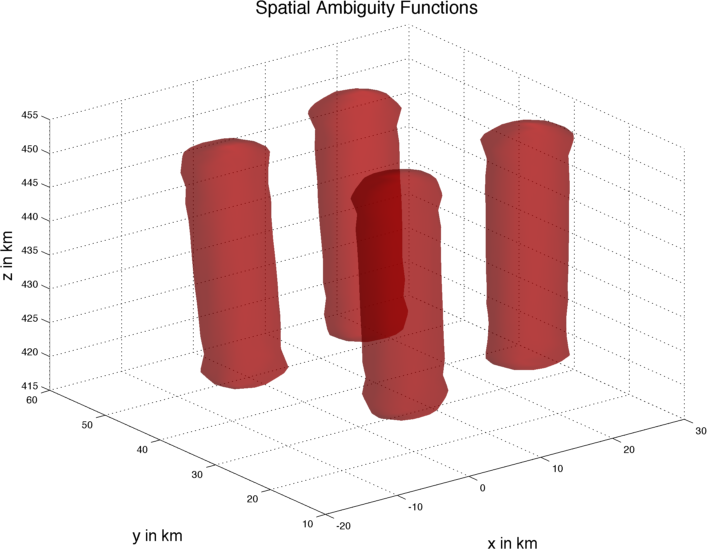
\includegraphics[width=5.5in]{spaceamb}
	\caption{Full Spatial Ambiguity Function}	
	\label{fig:amb4}
\end{figure}


\subsection{Ambiguity after Frame transformation}
In order to simplify notation first assume that the autocorrelation functions have been descritized and each $i^{th}$ lag can be represented as $x_i$. The measured lag product will also be represented as $y_i(\mathbf{r}_s,t_s)$. With this in mind the measurement process of the $i^{th}$ lag by the ISR can be represented as follows,

\begin{equation}
\label{eqn:firstL}
y_i(\mathbf{r}_s,t_s) = \int L_i(t_s,\mathbf{r}_s,t,\mathbf{r})x_i(t,\mathbf{r})dtd\mathbf{r}.
\end{equation}

For this we will focus on a single instance in the sampled time. We will assume that the radar is integrating over a length of time $T$ beginning at $t_0$ which will be the label of the sampled time. The operator $L$ will be represented as a separable function $KI$ where $I$ is an indicator function of length $T$ and centered at $t_0+1/2$. This will change (\ref{eqn:firstL}) to the following,

\begin{equation}
\label{eqn:L2}
y_{i,t_0}(\mathbf{r}_s) = \int K_i(\mathbf{r}_s,\mathbf{r})\int_{t_0}^{t_0+T} x_i(t,\mathbf{r})dtd\mathbf{r}.
\end{equation}

At this point it will be assumed that $x_i$ is rigid object and does not deform with respect to $\mathbf{r}$ over time period $[t_0,t_0+T]$. Also it will be assumed that the lag will be moving with a constant velocity $\mathbf{v}$. Thus $x_i(\mathbf{r},t)\Rightarrow x_i(\mathbf{r}+\mathbf{v}t)$. At this point (\ref{eqn:L2}) becomes,

\begin{equation}
\label{eqn:L3}
y_{i,t_0}(\mathbf{r}_s) = \int \int_{t_0}^{t_0+T} K_i(\mathbf{r}_s,\mathbf{r})x_i(\mathbf{r}+\mathbf{v}t)dtd\mathbf{r}.
\end{equation}

A change of variables where $\mathbf{r}' = \mathbf{r}+\mathbf{v}t$ acts as a Galilean transform and applies a warping to the kernel and changing the frame of reference. Then (\ref{eqn:L3}) becomes

\begin{equation}
\label{eqn:L4}
y_{i,t_0}(\mathbf{r}_s) = \int \int_{t_0}^{t_0+T} K_i(\mathbf{r}_s,\mathbf{r}'-\mathbf{v}t)x_i(\mathbf{r}')dtd\mathbf{r}'.
\end{equation}

The next step is to make the specific observation that in ISR each point of the sample spatial variable $\mathbf{r}_s$ will be the determined the $m^{th}$ range gate and the $n^{th}$ beam. This shows the final problem is truly a semi-discrete inverse problem and (\ref{eqn:L3}) becomes,

\begin{equation}
\label{eqn:L5}
y_{i,t_0,m,n}= \int \left[ \int_{t_0}^{t_0+T} K_{i,m,n}(\mathbf{r}'-\mathbf{v}t)dt \right]x_i(\mathbf{r}')d\mathbf{r}'.
\end{equation}

\noindent The kernel $K$ is actually a separable function with the component $f_{i,n}(\mathbf{r}')$ caused by the range ambiguity of the $i^{th}$ lag at the $m^{th}$ range gate. The function $g_m(\mathbf{r}')$ is the angle ambiguity from the $n^{th}$ beam. 

By performing the integration in $t$ the problem can now be simplified further back to a Friedholm integral equation by simply replacing the terms  in the square brackets as a new kernel $A$,

\begin{equation}
\label{eqn:L6}
y_{i,t_0,m,n}= \int A_{i,m,n}(\mathbf{r}') x_i(\mathbf{r}')d\mathbf{r}'.
\end{equation}
\noindent We are now left with a semi-discrete inverse problem to solve. The operator $A$ can be estimated through knowledge of the radar system and pulse pattern which would determine the antenna beam pattern and the range ambiguity function. The velocity $\mathbf{v}$ can be estimated by taking taking measurements of the Doppler shift and using a methodology seen in \cite{butler:imagingfregiondrifts}. Once the operator has been determined debluring methods can be applied.



\begin{figure}[!t]
	\centering
	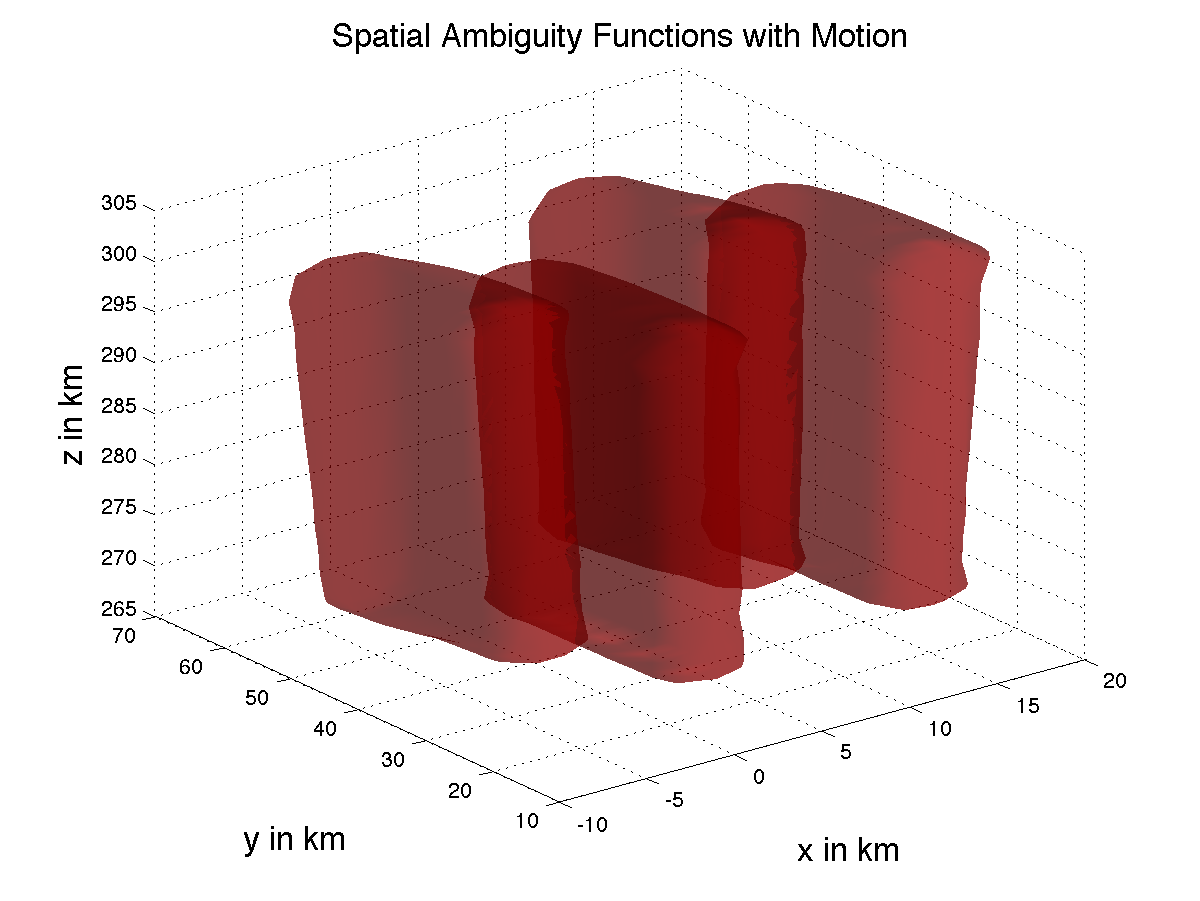
\includegraphics[width=5.5in]{spaceambmoving}
	\caption{Full Spatial Ambiguity Function With Motion}
	\label{fig:ambtime}
\end{figure}



%%%%%%%%%%%%%% Simulation %%%%%%%%%%%%%%%%%%%%%%%%%%%%%%%%%%%%%

\section{Simulation}
%%%%%%%%%%%%%% Mitigation %%%%%%%%%%%%%%%%%%%%%%%%%%%%%%%%%%%%%

\section{Possible Mitigation Techniques}
%%%%%%%%%%%%%% Conclusion %%%%%%%%%%%%%%%%%%%%%%%%%%%%%%%%%%%%

\section{Conclusion}
\bibliographystyle{BibTeX/agufull08}
\bibliography{BibTeX/litreview}

\begin{acknowledgments}
(Text here)
\end{acknowledgments}

\end{article}

\end{document}